\documentclass[tikz,border=8pt]{standalone}

\usepackage[T1]{fontenc}
\usepackage[utf8]{inputenc}
\usepackage{lmodern}
\usepackage{amsmath}
\usepackage{amssymb}
\usepackage{tikz}
\usetikzlibrary{arrows.meta,positioning,fit,calc,backgrounds}

\begin{document}
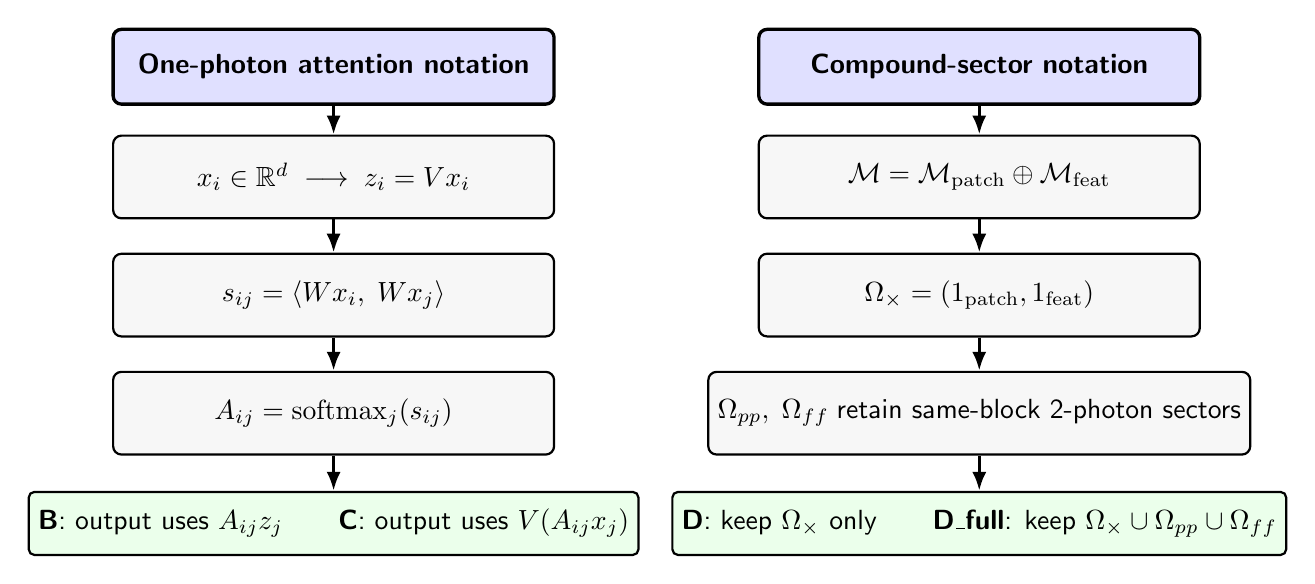
\begin{tikzpicture}[
  font=\sffamily,
  x=1cm, y=1cm,
  section/.style={draw, rounded corners=3pt, minimum width=5.6cm, minimum height=0.95cm, align=center, fill=blue!12, very thick},
  eqbox/.style={draw, rounded corners=3pt, minimum width=5.6cm, minimum height=1.05cm, align=center, fill=gray!6, thick},
  note/.style={draw, rounded corners=2pt, minimum width=5.6cm, minimum height=0.8cm, align=center, fill=green!8, thick},
  arrow/.style={-{Latex[length=2.4mm]}, very thick}
]

\node[section] (oneph) at (0, 0) {\textbf{One-photon attention notation}};
\node[eqbox]   (eq1)   at (0, -1.4) {$x_i \in \mathbb{R}^{d}\;\longrightarrow\; z_i = Vx_i$};
\node[eqbox]   (eq2)   at (0, -2.9) {$s_{ij} = \langle W x_i,\; W x_j\rangle$};
\node[eqbox]   (eq3)   at (0, -4.4) {$A_{ij} = \mathrm{softmax}_j(s_{ij})$};
\node[note]    (n1)    at (0, -5.8) {\textbf{B}: output uses $A_{ij} z_j$\qquad \textbf{C}: output uses $V(A_{ij}x_j)$};

\node[section] (comp)  at (8.2, 0) {\textbf{Compound-sector notation}};
\node[eqbox]   (ceq1)  at (8.2, -1.4) {$\mathcal{M} = \mathcal{M}_{\mathrm{patch}} \oplus \mathcal{M}_{\mathrm{feat}}$};
\node[eqbox]   (ceq2)  at (8.2, -2.9) {$\Omega_{\times} = (1_{\mathrm{patch}},1_{\mathrm{feat}})$};
\node[eqbox]   (ceq3)  at (8.2, -4.4) {$\Omega_{pp},\;\Omega_{ff}\;\text{retain same-block 2-photon sectors}$};
\node[note]    (n2)    at (8.2, -5.8) {\textbf{D}: keep $\Omega_{\times}$ only\qquad \textbf{D\_full}: keep $\Omega_{\times}\cup\Omega_{pp}\cup\Omega_{ff}$};

\draw[arrow] (oneph.south) -- (eq1.north);
\draw[arrow] (eq1.south) -- (eq2.north);
\draw[arrow] (eq2.south) -- (eq3.north);
\draw[arrow] (eq3.south) -- (n1.north);

\draw[arrow] (comp.south) -- (ceq1.north);
\draw[arrow] (ceq1.south) -- (ceq2.north);
\draw[arrow] (ceq2.south) -- (ceq3.north);
\draw[arrow] (ceq3.south) -- (n2.north);
\end{tikzpicture}
\end{document}
